
%%%%%%%%%%%%%%%%%%%%%%%%%%%%%%%%%%%%%%%%%%%%%%%%%%%%%%%%%%%%
%%  This Beamer template was created by Cameron Bracken.
%%  Anyone can freely use or modify it for any purpose
%%  without attribution.
%%
%%  Last Modified: January 9, 2009
%%

\documentclass[xcolor={x11names,table},compress,svgnames,mathserif]{beamer}

%% General document %%%%%%%%%%%%%%%%%%%%%%%%%%%%%%%%%%
\usepackage{graphicx}
\usepackage{tikz}
\usetikzlibrary{decorations.fractals}
%\usepackage{lmodern}
\usepackage{animate}
\usepackage{movie15}
\usepackage{bm}
\usepackage{pifont}
\usepackage{empheq}
\usepackage[many]{tcolorbox}
\usepackage{smartdiagram}
\usepackage[customcolors]{hf-tikz}
\usepackage{dashrule} % for dotted vertical line
\definecolor{airforceblue}{rgb}{0.36, 0.54, 0.66}
\definecolor{pigment}{rgb}{0.2, 0.2, 0.6}
%\usepackage{flexisym}

\usepackage[absolute,overlay]{textpos}

\pgfdeclarehorizontalshading{section shading}{2cm}{
color(0cm)=(LightSlateGrey);
color(2cm)=(gray!7);
color(3cm)=(LightSlateGrey!15)
}

% Custom block environment
% Custom block environment
\newenvironment<>{varblock}[2][.9\textwidth]{%
  \setlength{\textwidth}{#1}
  \begin{actionenv}#3%
    \def\insertblocktitle{#2}%
    \par%
    \usebeamertemplate{block begin}}
  {\par%
    \usebeamertemplate{block end}%
  \end{actionenv}}

% boxed equaton
\usepackage[many]{tcolorbox}
%\tcbuselibrary{skins}

\tcbset{highlight math style={enhanced,
  colframe=red!60!black,colback=yellow!50!white,arc=4pt,boxrule=1pt,
  }}

\newtcbox{\mybox}[1][]{nobeforeafter,math upper,tcbox raise base,
  enhanced,frame hidden,boxrule=0pt,interior style={top color=green!10!white,
  bottom color=green!10!white,middle color=green!50!yellow},
  fuzzy halo=1pt with green,drop large lifted shadow,#1}

%%%%%%%%%%%%%%%%%%%%%%%%%%%%%%%%%%%%%%%%%%%%%%%%%%%%%%

\usetikzlibrary{shapes,arrows}
\usetikzlibrary{positioning,decorations.pathreplacing}
% Define block styles
\tikzstyle{decision} = [diamond, draw, fill=purple!20, 
    text width=5.0em, text badly centered, node distance=3cm, inner sep=0pt]
\tikzstyle{block} = [rectangle, draw=none, fill=blue!20, anchor=north, 
    text width=9.0em, text centered]
    \tikzstyle{blockr} = [rectangle, draw, fill=blue!20, 
    text width=9.0em, text centered, rounded corners]
\tikzstyle{line} = [draw, -latex']
\tikzstyle{cloud} = [draw=none, ellipse,fill=purple!20, node distance=3cm,
    minimum height=2em]
    

%% Beamer Layout %%%%%%%%%%%%%%%%%%%%%%%%%%%%%%%%%%
\useoutertheme[subsection=false,shadow]{miniframes}
\useinnertheme{default}
%\usefonttheme{serif}
\usepackage{palatino}
\usepackage{xcolor}
\usepackage{amsmath}
\newcommand{\angstrom}{\textup{\AA}}

\setbeamerfont{title like}{shape=\scshape}
\setbeamerfont{frametitle}{shape=\scshape}
\setbeamertemplate{itemize items}[triangle] % if you wnat a circle
\setbeamertemplate{itemize subitem}[triangle]
\setbeamertemplate{navigation symbols}{}
%\setbeamertemplate{footline}[frame number]

\setbeamercolor{footlinecolor}{fg=white,bg=DeepSkyBlue4}
\defbeamertemplate*{footline}{infolines theme}
{
  \leavevmode%
  \hbox{%
  \begin{beamercolorbox}[wd=.333333\paperwidth,ht=2.25ex,dp=1ex,center]{footlinecolor}
 % {author in head/foot}%
    \usebeamerfont{author in head/foot}\insertshortauthor
   % \usebeamerfont{author in head/foot}\insertshortauthor~~(\insertshortinstitute)
  \end{beamercolorbox}%
  \begin{beamercolorbox}[wd=.333333\paperwidth,ht=2.25ex,dp=1ex,center]{title in head/foot}%
    \usebeamerfont{title in head/foot}\insertshorttitle
  \end{beamercolorbox}%
  \begin{beamercolorbox}[wd=.333333\paperwidth,ht=2.25ex,dp=1ex,right]{footlinecolor}
  %{date in head/foot}%
   % \usebeamerfont{date in head/foot}\insertshortdate{}\hspace*{2em}
    \usebeamerfont{date in head/foot}{manav.vohra@vanderbilt.edu}\hspace*{2em}
    \insertframenumber{} / \inserttotalframenumber\hspace*{2ex} 
  \end{beamercolorbox}}%
  \vskip0pt%
}
%\setbeamercolor{section in head/foot}{fg=white, bg=DeepSkyBlue4}

\setbeamercolor*{lower separation line head}{bg=DeepSkyBlue4} 
\setbeamercolor*{normal text}{fg=black,bg=white} 
\setbeamercolor*{alerted text}{fg=red} 
\setbeamercolor*{example text}{fg=black} 
\setbeamercolor*{structure}{fg=black} 
 
\setbeamercolor*{palette tertiary}{fg=black,bg=black!10} 
\setbeamercolor*{palette quaternary}{fg=black,bg=black!10} 

\renewcommand{\(}{\begin{columns}}
\renewcommand*\footnoterule{}
\renewcommand{\)}{\end{columns}}
\newcommand{\<}[1]{\begin{column}{#1}}
\renewcommand{\>}{\end{column}}

\newcommand*\subitem{%
  \item[\color{DeepSkyBlue4}\scalebox{0.6}{\ding{228}}]}
  
  \newcommand*\subitemtwo{%
  \item[\color{LightSlateGrey!15}\scalebox{0.6}{\ding{228}}]}

\newcommand*\myitem{%
  \item[\color{DeepSkyBlue4}\scalebox{0.6}{\ding{110}}]}
 
  \newcommand*\myitemtwo{%
  \item[\color{LightSlateGrey!15}\scalebox{0.6}{\ding{110}}]}
  
\newcommand*\Myitem{%
  \item[\color{DeepSkyBlue4}\scalebox{0.9}{\ding{42}}]}
  
\newcommand{\be}{\begin{equation}}
\newcommand{\ee}{\end{equation}}
\newcommand{\bea}{\begin{eqnarray}}
\newcommand{\eea}{\end{eqnarray}}
\newcommand{\p}{\partial}
\def\ol{\overline}
\def\no{\noindent}
\def\Vb{{\cal V}}
\def\Qd{\dot{Q}}
%\DeclareMathSymbol{\ast}{\mathbin}{symbols}{"03}
 \newcommand{\argmax}{\operatornamewithlimits{arg\,max}}

%-----------Parameter screening tikz styles -----------------------
   \tikzstyle{A} = [rectangle, rounded corners, minimum width=1.5cm, minimum height=0.5cm,text centered, draw=black,
     fill=blue!30]
      \tikzstyle{B} = [rectangle, rounded corners, minimum width=1.5cm, minimum height=0.5cm,text centered, draw=black,
     fill=red!30]
      \tikzstyle{p} = [rectangle, rounded corners, minimum width=1.5cm, minimum height=0.5cm,text centered, draw=black,
     fill=yellow!30]
      \tikzstyle{q} = [rectangle, rounded corners, minimum width=1.5cm, minimum height=0.5cm,text centered, draw=black,
     fill=green!30]
      \tikzstyle{alpha} = [rectangle, rounded corners, minimum width=1.5cm, minimum height=0.5cm,text centered, draw=black,
     fill=magenta!30]
      \tikzstyle{lambda} = [rectangle, rounded corners, minimum width=1.5cm, minimum height=0.5cm,text centered, draw=black,
     fill=cyan!30]
      \tikzstyle{gamma} = [rectangle, rounded corners, minimum width=1.5cm, minimum height=0.5cm,text centered, draw=black,
     fill=orange!30]
 \tikzstyle{outer} = [rectangle, minimum width=1.5cm, minimum height=0.5cm,text centered, draw=black,dashed]    
 \tikzstyle{pool} = [rectangle, minimum width=2.0cm, minimum height=1.6cm,line width=1pt,
text centered, draw=black,dashed]    

%% Algorithm %%%%%
\usepackage[linesnumbered]{algorithm2e}
\newcommand{\nosemic}{\renewcommand{\@endalgocfline}{\relax}}% Drop semi-colon ;
\newcommand{\dosemic}{\renewcommand{\@endalgocfline}{\algocf@endline}}% Reinstate semi-colon ;
\newcommand{\pushline}{\Indp}% Indent
\newcommand{\popline}{\Indm\dosemic}% Undent
\let\oldnl\nl% Store \nl in \oldnl
\newcommand{\nonl}{\renewcommand{\nl}{\let\nl\oldnl}}% Remove line number for one
\SetKwRepeat{Do}{do}{while}
%%%%%%%%%%%%%%%%%
 
%---------------------QUOTATION--------------------------
\usepackage{etoolbox}
%\usepackage[svgnames]{xcolor}
\usepackage{framed}

% conditional for xetex or luatex
\newif\ifxetexorluatex
\ifxetex
  \xetexorluatextrue
\else
  \ifluatex
    \xetexorluatextrue
  \else
    \xetexorluatexfalse
  \fi
\fi
%
\ifxetexorluatex%
  \usepackage{fontspec}
  \usepackage{libertine} % or use \setmainfont to choose any font on your system
  \newfontfamily\quotefont[Ligatures=TeX]{Linux Libertine O} % selects Libertine as the quote font
\else
  \usepackage[utf8]{inputenc}
  \usepackage[T1]{fontenc}
  %\usepackage{libertine} % or any other font package
  \newcommand*\quotefont{\fontfamily{LinuxLibertineT-LF}} % selects Libertine as the quote font
\fi

\newcommand*\quotesize{30} % if quote size changes, need a way to make shifts relative
% Make commands for the quotes
\newcommand*{\openquote}
   {\tikz[remember picture,overlay,xshift=-3ex,yshift=-0.5ex]
   \node (OQ) {\quotefont\fontsize{\quotesize}{\quotesize}\selectfont``};\kern0pt}

\newcommand*{\closequote}[1]
  {\tikz[remember picture,overlay,xshift=-15ex,yshift={#1}]
   \node (CQ) {\quotefont\fontsize{\quotesize}{\quotesize}\selectfont''};}

% select a colour for the shading
\colorlet{shadecolor}{Azure}

\newcommand*\shadedauthorformat{\emph} % define format for the author argument

% Now a command to allow left, right and centre alignment of the author
\newcommand*\authoralign[1]{%
  \if#1l
    \def\authorfill{}\def\quotefill{\hfill}
  \else
    \if#1r
      \def\authorfill{\hfill}\def\quotefill{}
    \else
      \if#1c
        \gdef\authorfill{\hfill}\def\quotefill{\hfill}
      \else\typeout{Invalid option}
      \fi
    \fi
  \fi}
% wrap everything in its own environment which takes one argument (author) and one optional argument
% specifying the alignment [l, r or c]
%
\newenvironment{shadequote}[2][l]%
{\authoralign{#1}
\ifblank{#2}
   {\def\shadequoteauthor{}\def\yshift{-2ex}\def\quotefill{\hfill}}
   {\def\shadequoteauthor{\par\authorfill\shadedauthorformat{#2}}\def\yshift{2ex}}
\begin{snugshade}\begin{quote}\openquote}
{\shadequoteauthor\quotefill\closequote{\yshift}\end{quote}\end{snugshade}}


%%%%%%%%%%%%%%%%%%%%%%%%%%%%%%%%%%%%%%%%%%%%%%%%%%

\title[UQ: Nano-scale Phonon Heat Transfer]{\textbf{Characterizing Errors and Uncertainties in
NEMD Simulations of Phonon Transport}}
\thispagestyle{empty}
\pgfsetfillopacity{0.9}
\setbeamercolor{title}{bg=DeepSkyBlue4,fg=white}


%\subtitle{SUBTITLE}
\author[M. Vohra and S. Mahadevan]{Manav Vohra$^{\dag}$, Sankaran Mahadevan$^{\dag}$ \\ \vspace{2mm}
\scriptsize{Collaborators: Seungha Shin$^{\S}$, Ali Y. Nobakht$^{\S}$}}
\vspace{-1mm}
\institute{$^{\dag}$Vanderbilt University\\ \vspace{1mm}
$^{\S}$University of Tennessee, Knoxville}

\date{\today}


\begin{document}


%___________________________NEW SLIDE______________________________________
{
\setbeamertemplate{headline}{}

\begin{frame}[noframenumbering]

\titlepage
\vspace{-21mm}
\centering
%\scriptsize Institute for Computational Engineering and Sciences\\ \vspace{1mm}
%The University of Texas at Austin \\ \vspace{6mm}

%\footnotesize Seminar at SCI, University of Utah \\ \vspace{2mm}


\end{frame}
}

%___________________________NEW SLIDE______________________________________

\section{\scshape Background}
\subsection{bg}

\begin{frame}{Non-Equilibrium MD}

\begin{itemize}

\myitem Widely used to study thermal (phonon) transport in 
{\color{pigment}non-metallic} systems (C,Si,Ge).
\vspace{2mm}
\myitem System subjected to a temperature gradient using thermostats.
\vspace{2mm}
\myitem {\color{pigment}Steady-state} thermal energy exchange between
the thermostats is used in Fourier's law to estimate bulk thermal
conductivity~($\kappa$). \vspace{2mm}
\myitem Estimates are {\color{pigment}uncertain} and severely
{\color{pigment}under-predicted}.
\begin{itemize}
  \item Simulation length-scales $\ll$ phonon mean free path. \vspace{1mm}
  \item Thermostats reduce correlation b/w vibration modes.
\end{itemize}

\end{itemize}

\end{frame}

%___________________________NEW SLIDE______________________________________

\subsection{bg}

\begin{frame}{Sources of Uncertainty}

\begin{columns}
\begin{column}{0.52\textwidth}

\begin{itemize}
\myitem Bulk thermal conductivity is size-dependent.
\vspace{2mm}
\myitem Variability in applied thermal gradient~(Kapitza~effect).
\vspace{2mm}
\myitem Choice of the inter-atomic potential.
\vspace{2mm}
\myitem Nominal estimates of the potential parameters.

\end{itemize}
\end{column}

\begin{column}{0.48\textwidth}

\begin{center}
\begin{figure}[htbp]
\vspace{-3mm}
  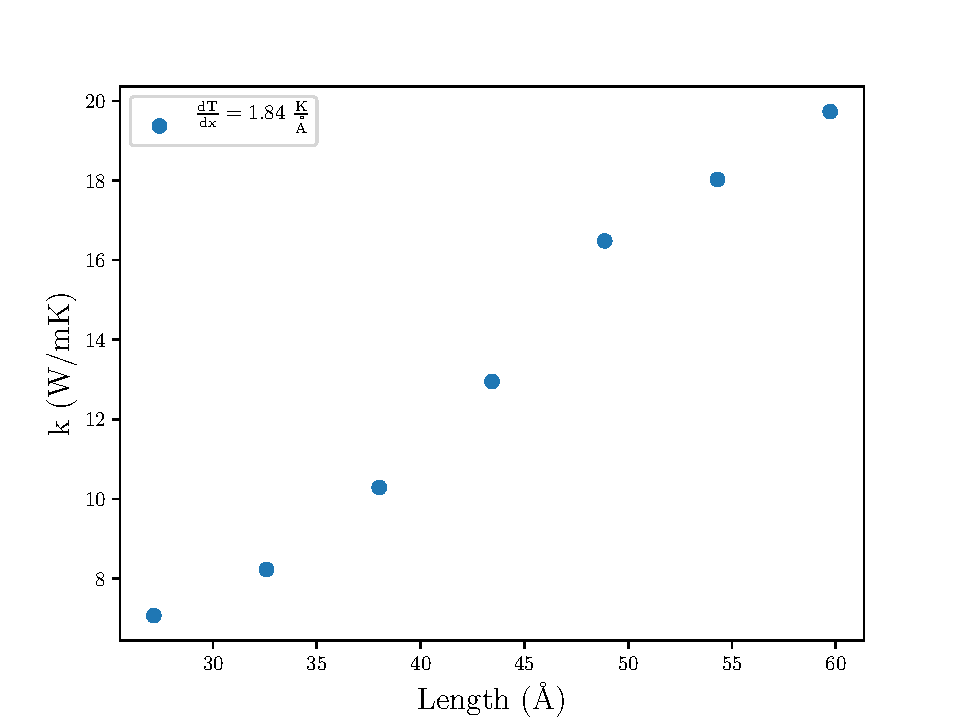
\includegraphics[width=0.9\textwidth]{./Figures/cond_size}
  \\ \vspace{2mm}
  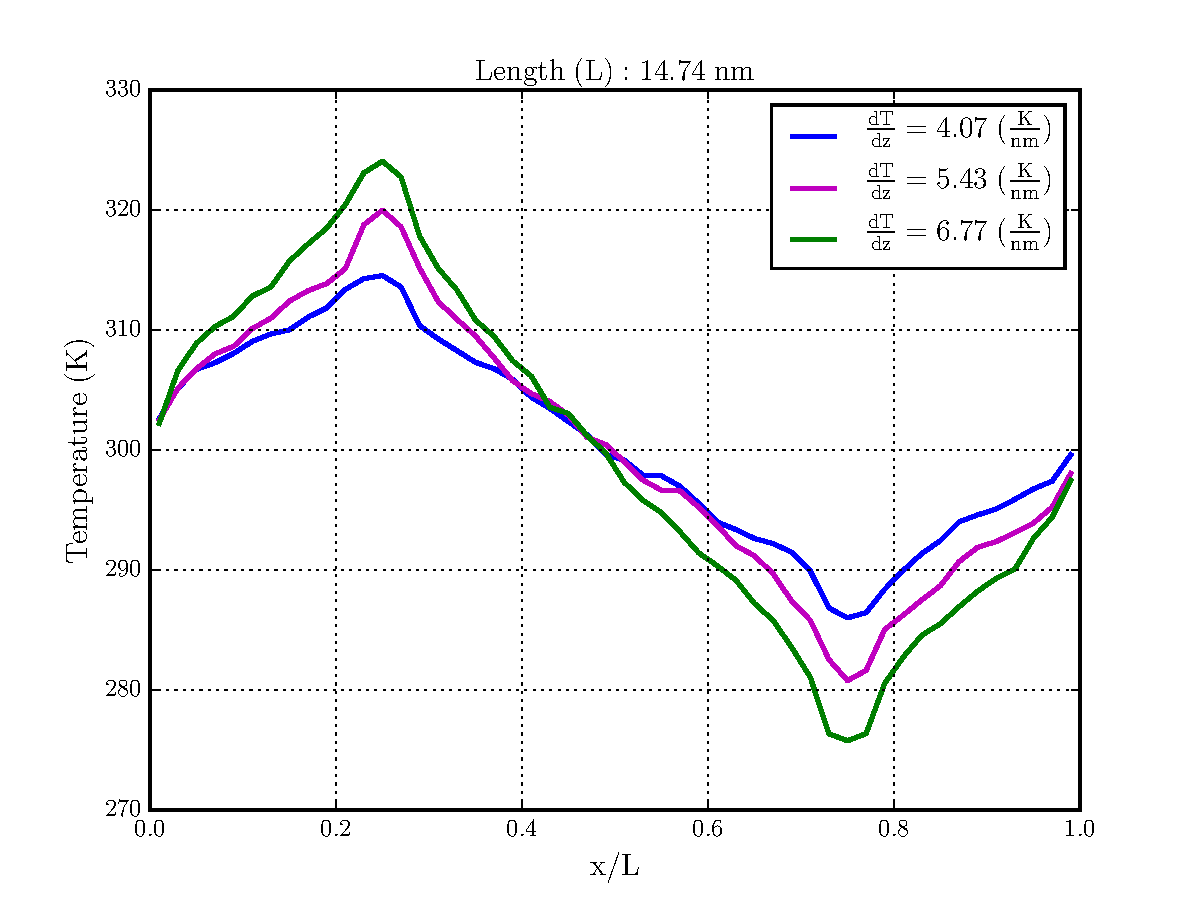
\includegraphics[width=0.9\textwidth]{./Figures/temp_plot}
\end{figure}
\end{center}

\end{column}
\end{columns}


\end{frame}

%___________________________NEW SLIDE______________________________________

\subsection{bg}

\begin{frame}{Specific Research Goals}

\begin{itemize}

\myitem Quantify discrepancy in $\kappa$ between predictions and data.
\begin{itemize}
\item Construct a response surface for $\kappa(s,\frac{d\theta}{dx})$.
\end{itemize}
\vspace{2mm}
\myitem Perform sensitivity analysis of the potential parameters.
\begin{itemize}
\item Estimate derivative-based sensitivity measures~(DGSM).
\end{itemize}
\vspace{2mm}
\myitem Construct a reduced order surrogate for $\kappa$ using sparse
NEMD predictions.
\begin{itemize}
\item Use the surrogate for forward propagation of uncertainty, and global
sensitivity analysis. 
\end{itemize}
\vspace{2mm}
\myitem Calibrate the \textit{important} parameters in a Bayesian setting.

\end{itemize}

\end{frame}

%___________________________NEW SLIDE______________________________________

\section{\scshape Set-up}
\subsection{setup}

\begin{frame}{Problem Set-up}

\begin{columns}
\begin{column}{0.5\textwidth}

\begin{center}
\begin{tikzpicture}
\node[fill=white,inner sep=0pt] 
{\rowcolors{1}{DeepSkyBlue!20}{DeepSkyBlue!5}
	\resizebox{\columnwidth}{!}{
  \begin{tabular}{l|c}
%\hline
	Lattice Constant, $a$ ($\angstrom$) & 5.43 \\ 
	Width, Height ($\angstrom$) & 22$a$ \\ 
	$\Delta t$  (ps) & 0.0005 \\
	Boundary Condition & Periodic \\ 
	Lattice Structure & Diamond \\ 
	Inter-atomic Potential & Stillinger-Weber 

%\hline
  \end{tabular}%
	}
};
\end{tikzpicture}
\end{center}

\end{column}

\begin{column}{0.5\textwidth}

%\vspace{-5mm}
\begin{center}
\begin{figure}[htbp]
        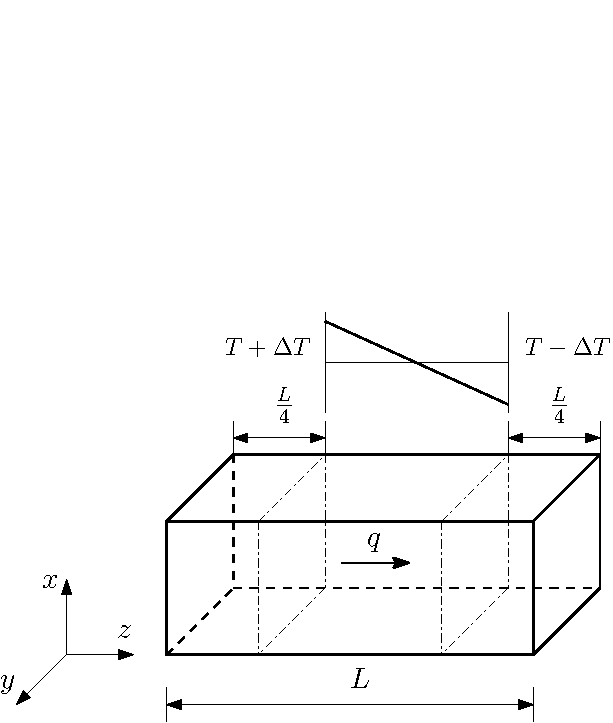
\includegraphics[width=0.9\textwidth]{./Figures/schematic}
\end{figure}
\vspace{3mm}
%        \animategraphics[autopause,poster=first,loop,height=0.60\textwidth]{5}
%        {./animation/snap}{0}{64}
\end{center}
\end{column}
\end{columns}

\end{frame}

%___________________________NEW SLIDE______________________________________

\subsection{setup}
\begin{frame}{Problem Set-up}

%\vspace{-4mm}

\begin{itemize}
\myitem \textsc{Stages}:\\

\begin{center}
{\color{green}NVT} \hspace{5mm} $\rightarrow$ \hspace{5mm} {\color{cyan}NVE} \hspace{5mm}
$\rightarrow$ \hspace{5mm} {\color{magenta}NVE}
\\ \vspace{1mm}
\tiny \hspace{-5mm}[Eqilibrate system to 300 K] \hspace{1mm} [Equilibrate thermostats] \hspace{4mm}
 [Generate Data]
\\ \vspace{1mm}

\tiny{N: Number of Atoms~~~V: Volume~~~T: Temperature~~~E: Energy}
\end{center}

\normalsize

\myitem \textsc{Observable}: Avg. energy exchange b/w thermostats~($q$)
\vspace{2mm}

\myitem \textsc{QoI}: Bulk thermal conductivity ($\kappa$)

\begin{empheq}[box=\tcbhighmath]{align}
  \kappa = \frac{q}{\left|\frac{dT}{dx}\right|} \nonumber
\end{empheq}

\vspace{2mm}

\myitem Appropriate selection of {\color{pigment}width}, 
{\color{pigment}height}, and {\color{pigment}simulation-time} was ensured.  
\end{itemize}

\end{frame}

%___________________________NEW SLIDE______________________________________

\section{\scshape Discrepancy}
\subsection{response}
\begin{frame}{Response Surface: Discrepancy}

\begin{columns}
\begin{column}{0.52\textwidth}

\begin{itemize}
\myitem PC representation of the discrepancy, 
$\epsilon_{\mbox{\tiny{d}}}$:

\begin{empheq}[box=\tcbhighmath]{align}
\epsilon_{\mbox{\tiny{d}}} \approx \mathcal{\epsilon}_{\mbox{\tiny{d}}}^{\mbox{\tiny{PCE}}} = 
\sum_{\bm{k}\in\mathcal{I}} c_{\bm{k}}(T)\Psi_{\bm{k}}(\bm{\xi(\theta)})
\nonumber
\end{empheq}

\end{itemize}
\end{column}

\begin{column}{0.48\textwidth}

\begin{center}
\begin{figure}[htbp]
\vspace{-3mm}
  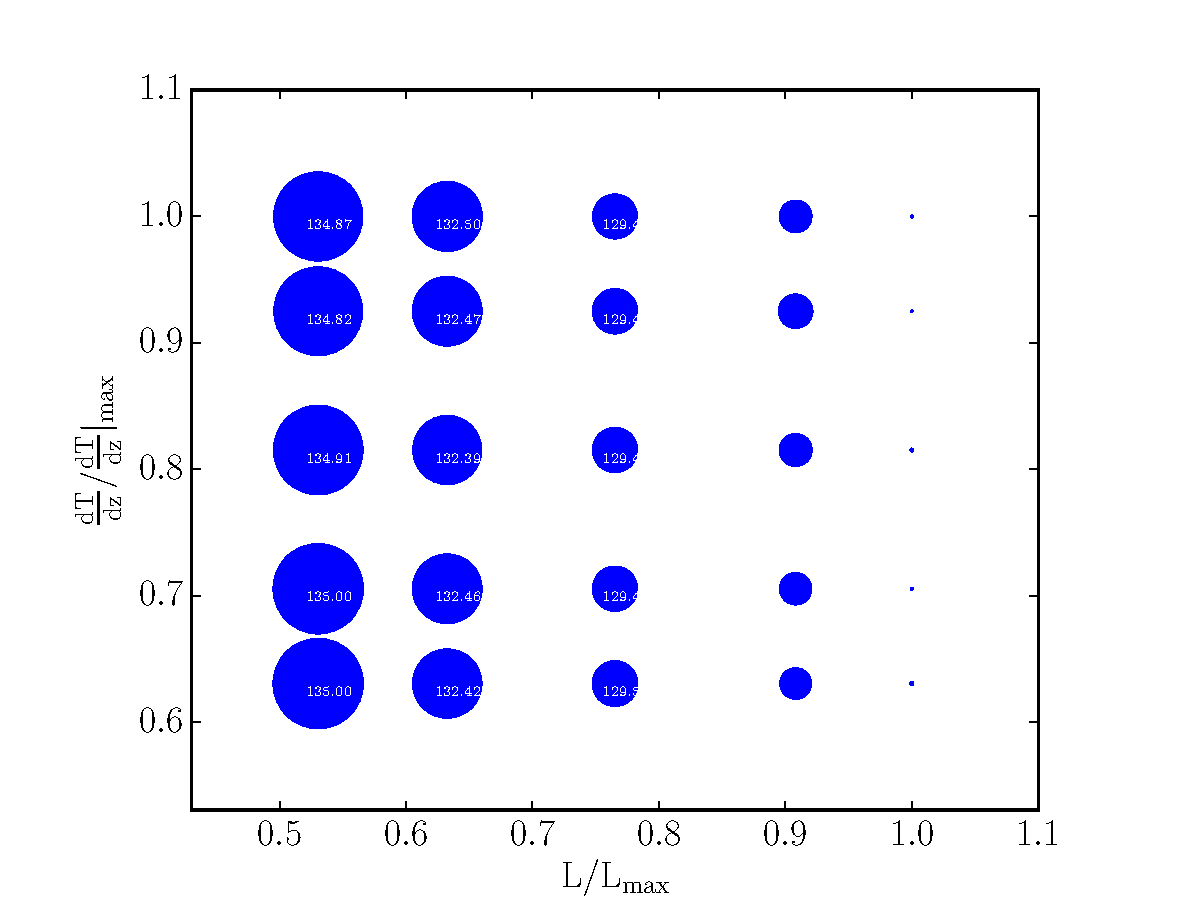
\includegraphics[width=0.95\textwidth]{./Figures/realz_quad300K}
  \\ \vspace{1mm}
  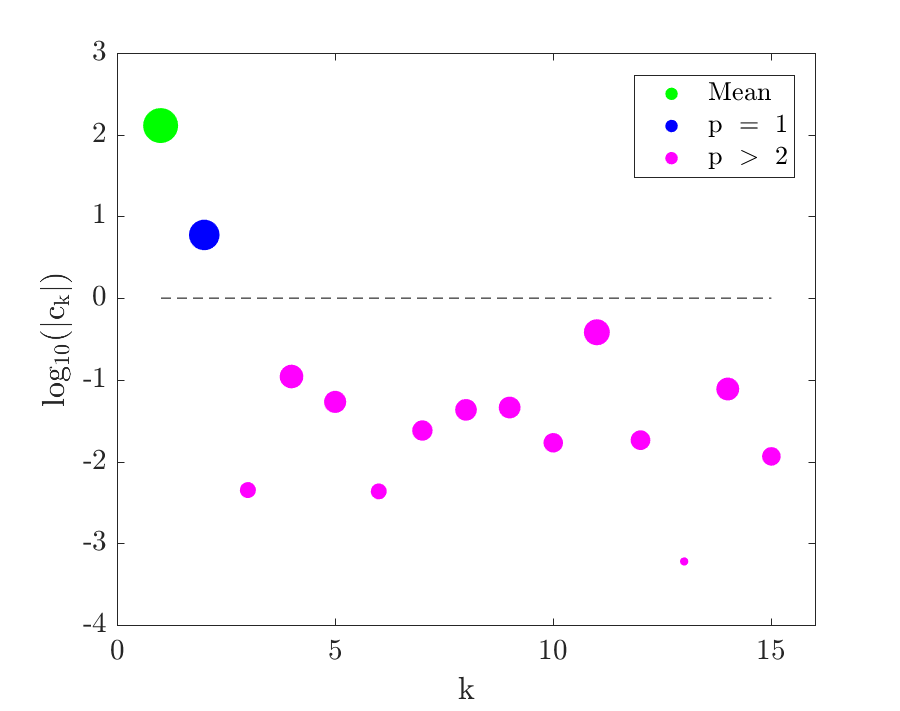
\includegraphics[width=0.9\textwidth]{./Figures/PCspectrum_300}
\end{figure}
\end{center}

\end{column}
\end{columns}

\end{frame}




































\end{document}
